\documentclass{presentation}

\usepackage{tikz}
\usepackage{pausegraphics}

\newcommand{\rect}[1]{\tikz{\path[draw=black,fill=#1] (0,0) rectangle (2mm,2mm);}}
\newcommand{\grect}{\rect{white!60!green}}
\newcommand{\rrect}{\rect{white!60!red}}
\newcommand{\wrect}{\rect{white}}
\newcommand{\brect}{\rect{gray}}

% some details about the cover page
\title[slide $\text{\insertframenumber}$]{Efficient Algorithm}
\subtitle{Jump points}
\author{Rademacher, Loka}
\date{\today}
\institute{
    Department of Computer Science \\
    University of Bonn
}

\begin{document}


\begin{frame}
    \titlepage
\end{frame}



\begin{frame}{Contents}
    \begin{itemize}
        \item Path finding on grid graphs
        \item A Star Search ($A^\star$)
        \item Jump Point Search ($JPS$)
        \item Jump Point Search Improvements ($JPS^+$)
        \item Bounding Boxes ($BB$)
        \item Defined goal
    \end{itemize}
\end{frame}



\begin{frame}
    \bigbox{Path finding on grid graphs}
\end{frame}

\begin{frame}{Problem definition}
	\begin{minipage}{0.3\textwidth}

	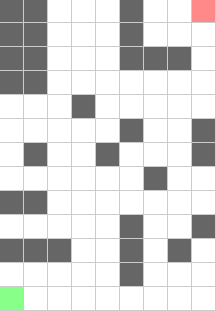
\includegraphics[width=\textwidth]{figures/gridgraph.png}

	\end{minipage}%
	\hfill%
	\begin{minipage}{0.6\textwidth}

	\begin{itemize}
		\item 4-tuple $(G, s, g, h)$:
		\pause
		\begin{itemize}
		\item[$\wrect$] Euclidean grid graph $G$
		\item[$\grect$] start node $s$
		\item[$\rrect$] goal node $g$
		\item[$\brect$] $\not\in G$ obstacle
		\pause
		\item[$\rightarrow$] edge costs $1$
		\item[$\nearrow$] edge costs $\sqrt{2}$
		\pause
		\item[$h$:] a heuristic function
		\end{itemize}
	\end{itemize}

	\end{minipage}

	\hspace{3cm}

	\pause
	\begin{center}
		Goal: shortest path from $s$ to $g$ over $G$
	\end{center}

\end{frame}


\begin{frame}{Heuristic Function $h$}
	\begin{minipage}{0.3\textwidth}
		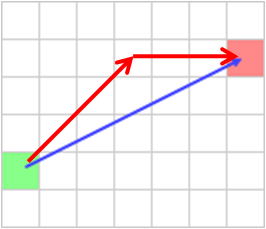
\includegraphics[width=\textwidth]{figures/heuristic.png}
	\end{minipage}%
	\hfill%
	\begin{minipage}{0.6\textwidth}
		\begin{itemize}
		\item let $\grect$ and $\rrect$ be arbitrary nodes
		\pause
		\item $h(\grect, \rrect)\leq min_{path}(\grect,\rrect)$
		\pause
		\item e.g.:\\ $h(\grect, \rrect) = dist_{euklid}(\grect,\rrect)$
		\begin{itemize}
			\item $\sqrt{27} \leq 3+3\cdot\sqrt{2}$
		\end{itemize}
		\end{itemize}
	\end{minipage}
\end{frame}


\begin{frame}
    \bigbox{A Star search ($A^\star$)}
\end{frame}


\begin{frame}{Main ideas: Neighborhood}
	\begin{center}
		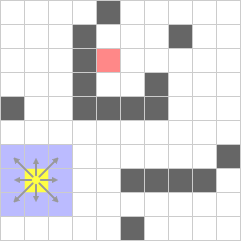
\includegraphics[width=0.5\textwidth]{figures/A-Stern_geschnitten(241x241)/2.png}
	\end{center}
\end{frame}


\begin{frame}{Main ideas: Priority Queue}
    %\begin{itemize}
    %    \item Frontier of nodes in a priority queue
    %    \item Value of a node is cost so far + heuristic to goal node
	%\end{itemize}


	q = square root of 2
	\vspace{1cm}

	5q - 3q+2 - 3q+2\\
	4q + 2 - start - 2q + 4\\
	5q + 2 - 3q + 4 - 3q + 4

	\vspace{1cm}
	so müsste das bild aussehen (auf 1 nachkommastelle runden)
\end{frame}


\begin{frame}{$A^*$: Example}
	\begin{minipage}{0.20\textwidth}
		\includegraphicspaused[width=\textwidth]{figures/A-Stern_geschnitten(241x241)/3.png}
	\end{minipage}%
	\pause%
	\hfill%
	\begin{minipage}{0.20\textwidth}
		\includegraphicspaused[width=\textwidth]{figures/A-Stern_geschnitten(241x241)/4.png}
	\end{minipage}%
	\pause%
	\hfill%
	\begin{minipage}{0.20\textwidth}
		\includegraphicspaused[width=\textwidth]{figures/A-Stern_geschnitten(241x241)/5.png}
	\end{minipage}\\
	\pause%

	\vspace{2mm}
	\begin{minipage}{0.20\textwidth}
		\includegraphicspaused[width=\textwidth]{figures/A-Stern_geschnitten(241x241)/6.png}
	\end{minipage}%
	\pause%
	\hfill%
	\begin{minipage}{0.20\textwidth}
		\includegraphicspaused[width=\textwidth]{figures/A-Stern_geschnitten(241x241)/7.png}
	\end{minipage}%
	\pause%
	\hfill%
	\begin{minipage}{0.20\textwidth}
		\includegraphicspaused[width=\textwidth]{figures/A-Stern_geschnitten(241x241)/8.png}
	\end{minipage}
	\pause%

	\vspace{2mm}
	\begin{minipage}{0.20\textwidth}
		\includegraphicspaused[width=\textwidth]{figures/A-Stern_geschnitten(241x241)/9.png}
	\end{minipage}%
	\pause%
	\hfill%
	\begin{minipage}{0.20\textwidth}
		\includegraphicspaused[width=\textwidth]{figures/A-Stern_geschnitten(241x241)/10.png}
	\end{minipage}%
	\pause%
	\hfill%
	\begin{minipage}{0.20\textwidth}
		\includegraphicspaused[width=\textwidth]{figures/A-Stern_geschnitten(241x241)/11.png}
	\end{minipage}%
\end{frame}


\begin{frame}
    \bigbox{Jump Point Search ($JPS$)}
\end{frame}


\begin{frame}{Main ideas: Symmetric paths}
	\begin{center}
		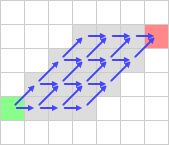
\includegraphics[width=0.5\textwidth]{figures/symmetricpath.png}\\
		\vspace{1cm}
		Diagonal First!
	\end{center}
\end{frame}


\begin{frame}{Main ideas: Exploring Rules \& Jump Points}
	\begin{center}
		Straight Movements:\\
		\vspace{5mm}
		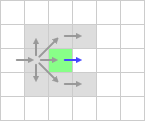
\includegraphics[width=0.5\textwidth]{figures/extra_geschnitten/sm.png}
	\end{center}
\end{frame}


\begin{frame}{Main ideas: Exploring Rules \& Jump Points}
		\begin{center}
		Straight Movements:\\
		\vspace{5mm}
		\begin{minipage}{0.3\textwidth}
			\includegraphicspaused[width=\textwidth]{figures/extra_geschnitten/sm(long).png}
		\end{minipage}%
		\pause%
		\hfill%
		\begin{minipage}{0.3\textwidth}
			\includegraphicspaused[width=\textwidth]{figures/extra_geschnitten/sm(obstacle).png}
		\end{minipage}%
		\pause%
		\hfill%
		\begin{minipage}{0.3\textwidth}
			\includegraphicspaused[width=\textwidth]{figures/extra_geschnitten/sm(forced).png}
		\end{minipage}%
	\end{center}
\end{frame}


\begin{frame}{Main ideas: Exploring Rules \& Jump Points}
	\begin{center}
		Diagonal Movements:\\
		\vspace{5mm}
		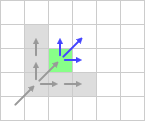
\includegraphics[width=0.5\textwidth]{figures/extra_geschnitten/dm.png}
	\end{center}
\end{frame}


\begin{frame}{Main ideas: Exploring Rules \& Jump Points}
		\begin{center}
		Diagonal Movements:\\
		\vspace{5mm}
		\begin{minipage}{0.3\textwidth}
			\includegraphicspaused[width=\textwidth]{figures/extra_geschnitten/dm(obstacle).png}
		\end{minipage}%
		\pause%
		\hfill%
		\begin{minipage}{0.3\textwidth}
			\includegraphicspaused[width=\textwidth]{figures/extra_geschnitten/dm(forced).png}
		\end{minipage}%
		\pause%
		\hfill%
		\begin{minipage}{0.3\textwidth}
			\includegraphicspaused[width=\textwidth]{figures/extra_geschnitten/dm(jump).png}
		\end{minipage}%
	\end{center}
\end{frame}


\begin{frame}{$JPS$: Example}
	\begin{minipage}{0.20\textwidth}
		\includegraphicspaused[width=\textwidth]{figures/jps_geschnitten/1.png}
	\end{minipage}%
	\pause%
	\hfill%
	\begin{minipage}{0.20\textwidth}
		\includegraphicspaused[width=\textwidth]{figures/jps_geschnitten/2.png}
	\end{minipage}%
	\pause%
	\hfill%
	\begin{minipage}{0.20\textwidth}
		\includegraphicspaused[width=\textwidth]{figures/jps_geschnitten/3.png}
	\end{minipage}%
	\pause%

	\vspace{2mm}

	\begin{minipage}{0.20\textwidth}
		\includegraphicspaused[width=\textwidth]{figures/jps_geschnitten/4.png}
	\end{minipage}%
	\pause%
	\hfill%
	\begin{minipage}{0.20\textwidth}
		\includegraphicspaused[width=\textwidth]{figures/jps_geschnitten/5.png}
	\end{minipage}%
	\pause%
	\hfill%
	\begin{minipage}{0.20\textwidth}
		\includegraphicspaused[width=\textwidth]{figures/jps_geschnitten/6.png}
	\end{minipage}%
	\pause%

	\vspace{2mm}

	\begin{minipage}{0.20\textwidth}
		\includegraphicspaused[width=\textwidth]{figures/jps_geschnitten/8.png}
	\end{minipage}%
	\pause%
	\hfill%
	\begin{minipage}{0.20\textwidth}
		\includegraphicspaused[width=\textwidth]{figures/jps_geschnitten/9.png}
	\end{minipage}%
	\pause%
	\hfill%
	\begin{minipage}{0.20\textwidth}
		\includegraphicspaused[width=\textwidth]{figures/jps_geschnitten/13.png}
	\end{minipage}
\end{frame}


\begin{frame}{$A^*$ vs. $JPS$}
	\begin{minipage}{0.45\textwidth}
		$A^*$:\\
		\vspace{3mm}
		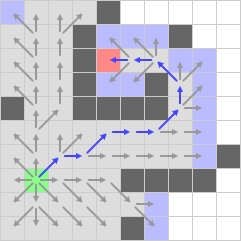
\includegraphics[width=\textwidth]{figures/A-Stern_geschnitten(241x241)/11.png}
	\end{minipage}%
	\hfill%
	\begin{minipage}{0.45\textwidth}
		$JPS$:\\
		\vspace{3mm}
		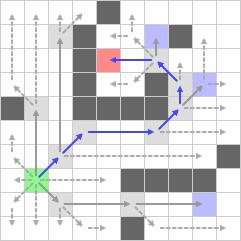
\includegraphics[width=\textwidth]{figures/jps_geschnitten/13.png}
	\end{minipage}
\end{frame}


\begin{frame}
    \bigbox{Jump Point Search Improvements ($JPS^+$)}
\end{frame}



\begin{frame}{Main ideas: Preprocessing Jump Points}
	\begin{minipage}{0.45\textwidth}
		Position of $\tikz{\path[draw=black,fill=yellow] (0,0) rectangle (2mm,2mm);}$:\\
		\vspace{3mm}
		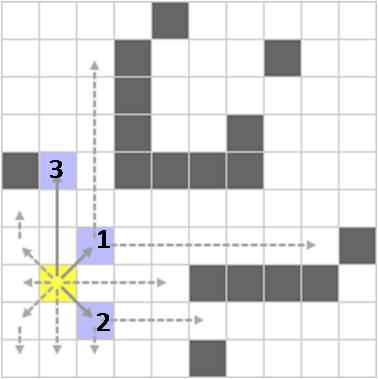
\includegraphics[width=\textwidth]{figures/jps_geschnitten/1(yellow).png}
	\end{minipage}%
	\hfill%
	\begin{minipage}{0.45\textwidth}
		Look up table for $\tikz{\path[draw=black,fill=yellow] (0,0) rectangle (2mm,2mm);}$:\\
		\vspace{3mm}
		\begin{itemize}
		\pause
		\item[$\nearrow$] $[\ 1\ ,\ path(\tikz{\path[draw=black,fill=yellow] (0,0) rectangle (2mm,2mm);}\ ,1)=\sqrt{2}\ ]$
		\pause
		\item[$\searrow$] $[\ 2\ ,\ path(\tikz{\path[draw=black,fill=yellow] (0,0) rectangle (2mm,2mm);}\ ,2)=\sqrt{2}\ ]$
		\item[$\swarrow$]
		\item[$\nwarrow$]
		\item[$\leftarrow$]
		\item[$\rightarrow$]
		\pause
		\item[$\uparrow$] $[\ 3\ ,\ path(\tikz{\path[draw=black,fill=yellow] (0,0) rectangle (2mm,2mm);}\ ,3)=3\ ]$
		\item[$\downarrow$]
		\end{itemize}
	\end{minipage}
\end{frame}


\begin{frame}
    \bigbox{Bounding Boxes ($BB$)}
\end{frame}



\begin{frame}{Description}
    \begin{itemize}
        \item Pruning technique
        \item Prepossessing offline
        \item A bounding box for each pair of node and direction

    \end{itemize}
\end{frame}


\begin{frame}{Box}
    \begin{itemize}
        \item Every node $n$ with an optimal path from $s$ to $n$ through this one must be contained by the box
        \item The box is the smallest bounding satisfying this
        \item Special treatment on JPS
    \end{itemize}
\end{frame}


\begin{frame}{Example}
    \begin{center}
        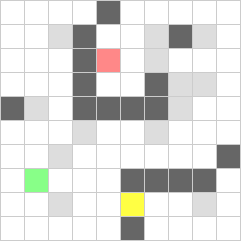
\includegraphics[width=0.5\textwidth]{figures/bounding_boxes1.png}
    \end{center}
\end{frame}


\begin{frame}{Example}
    \begin{center}
        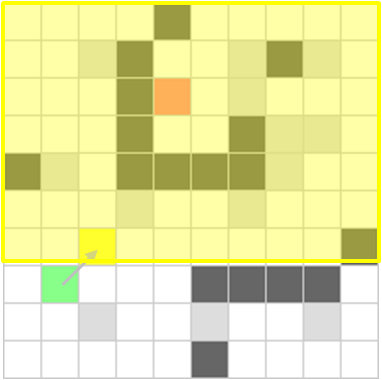
\includegraphics[width=0.5\textwidth]{figures/bounding_boxes2.png}
    \end{center}
\end{frame}



\begin{frame}
    \bigbox{Defined goal}

    Das können wir eigentlich weglassen
\end{frame}



\begin{frame}
    \bigbox{Thanks for attention!}
\end{frame}


\end{document}
